\documentclass[a4paper,12pt]{article}
\usepackage{graphicx}
\usepackage{cmap}
\usepackage[T2A]{fontenc}
\usepackage[utf8]{inputenc}
\usepackage{indentfirst}

%%\renewcommand{\footrulewidth}{ .0em }
\usepackage[english,russian]{babel}
\usepackage{multirow} % Слияние строк в таблице
\newcommand
{\un}[1]
{\ensuremath{\text{#1}}}




\begin{document}

\begin{titlepage}
	\begin{center}
		\large 	Московский физико-технический университет \\
		Физтех-школа радиотехники и компьютерных технологий\\
		\vspace{0.2cm}
		
		\vspace{4.5cm}
		Лабораторная работа № 3.4.5 \\ \vspace{0.2cm}
		\LARGE \textbf{Петля гистерезиса
		(динамический метод)}
	\end{center}
	\vspace{2.3cm} \large
	
	\begin{center}
		Работу выполнил: \\
		Орловский Антон \\
		Б01-909

		
	\end{center}
	
	\begin{center} \vspace{60mm}
		г. Долгопрудный \\
		 2020 год
	\end{center}
\end{titlepage}




\section{Цель работы} Исследование петель гистерезиса ферромагнитных материалов с помощью осциллографа.

\textbf{В работе используются:} \textit{понижающий трансформатор, реостат, амперметр и вольтметр (мультиметры), резистор, делитель напряжения, интегрирующая цепочка, электронный осциллограф, тороидальные образцы с двумя обмотками.}
	
\section{Теоретическая часть}		 
	Магнитную индукцию удобно определять с помощью ЭДС, возникающей при изменении магнитного потока $\Phi$ в катушке, намотанной на образец: $~~\mathscr{E}=-\frac{d\Phi}{dt}$.
	
	Пусть катушка плотно обхватывает образец, и индукция $\textbf{B}$
	в образце однородна. Тогда $\Phi=BSN$, где $N$ - число витков в измерительной катушке, а $S$ -- число витков.
	Подставим $\Phi$ в формулу ЭДС, после интегрирования найдем:
	$$|B|=\frac{1}{SN}\int\mathscr{E} dt$$
	
	Таким образом, для определения $B$ нужно проинтегрировать сигнал, наведенный меняющимся магнитным полем на измерительную катушку, намотанную на образец.
	
	Для интегрирования сигнала применяют интегрирующие схемы. На рис.1 изображена простейшая из них. При этом сопротивление $R$ заметно превышает сопротивление конденсатора ($U_{\text{вых}}\ll U_{\text{вх}}$).
		
	\begin{center}
	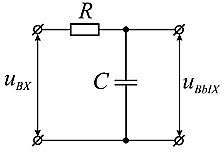
\includegraphics[width = 0.3\textwidth]{pic1.png}
	\end{center}
	
	В данном случае $I \approx U_{\text{вх}}/R$, а напряжение на емкости $$U_{\text{вых}}=\cfrac{q}{C}=\frac{1}{C}\int Idt \approx \frac{1}{RC}\int U_{\text{вх}}dt$$
	
	Чем больше постоянная времени $\tau =RC$ превосходит характерное время процесса, тем этот вывод ближе к истине. Для синусоидальных напряжений $U${\scriptsize вых}$=U${\scriptsize вх}$/RC\Omega$, где $\Omega$ - частота сигнала.
	
	Обозначив параметры интегрирующей ячейки через $R_{\text{и}}, C_{\text{и}}, N_{\text{и}}$, получим: $$|B|=\cfrac{R_{\text{и}}C_{\text{и}}}{SN_{\text{и}}}U_{\text{вых}}$$

%%newpage

\section{Экспериментальная установка}

Ток в обмотке $N_0$ измеряется мультиметром А. Напряжение с сопротивления $R_0$, включенного последовательно с обмоткой $N_0$, подается на вход $X$ электронного осциллографа (ЭО). Это напряжение пропорционально току в обмотке $N_0$, а следовательно, и напряженности $H$ магнитного поля в образце. 

Для измерения магнитной индукции $B$ с измерительной обмотки $N_i$ на вход интегрирующей $NC$-цепочки подается напряжение $U_{BX}$, пропорциональное производной $B$, а с выхода снимается напряжение $U_{EX}=U_C$, пропорциональное $B$ и подается на вход $Y$.

Замкнутая кривая, возникающая на экране, воспроизводит в некотором масштабе (различном для $X$ и $Y$) петлю гистерезиса.Необходимо провести калибровку каналов $X$ и $Y$ ЭО и установить масштабы изображения. Для этого надо узнать, каким напряжениям (или токам) соответствуют амплитуды сигналов, видимых на экране, и каким значениям $B$ и $H$ соответствуют напряжения (или токи).
\begin{center}
	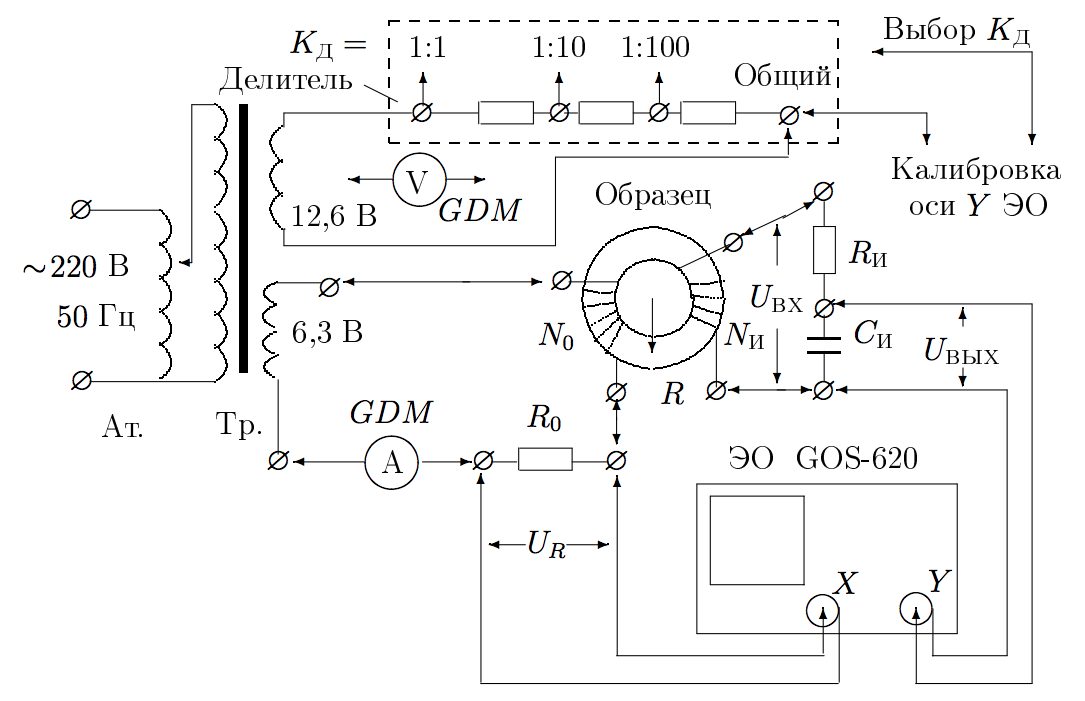
\includegraphics[width = 0.8\textwidth]{345-1.png}
\end{center}\

\textbf{Для измерения напряжения с помощью осциллографа:}

\begin{equation}\label{}
    2U_{X,0}=2x\cdot K_X; \hspace{2cm} 2U_{Y,0}=2y\cdot K_Y;
\end{equation}

\begin{equation}\label{}
    H=\frac{IN_0}{2\pi R}
\end{equation}

\begin{equation}\label{}
    |B|=\frac{R_u \cdot C_u}{SN_u}U_{ex}
\end{equation}


\textbf{Проверка калибровки горизонтальной оси ЭО с помощью амперметра:} (при закороченной обмотке $N_0$) 


\begin{equation}\label{}
    m_X=2R_0\sqrt{2}I_{ef}/(2x) 
\end{equation}

\textbf{Проверка калибровки вертикальной оси ЭО с помощью вольтметра:} (при отключенном тороиде)


\begin{equation}\label{}
    m_X=2R_0\sqrt{2}I_{ef}/(2x) 
\end{equation}


\textbf{Для измерения постоянной времени $RC$-цепочки:}

\begin{equation}\label{}
    \tau=RC=\frac{U_{in}}{\Omega U_{ex}}
\end{equation}


\bigskip


\section{Ход работы}

\subsection{Петля гистерезиса на экране ЭО}


Соберем схему согласно рисунку выше, подготовим приборы к работе и включим схему в сеть. Подберем ток питания в намагничивающей обмотке и коэффициенты усиления ЭО, так, чтобы предельная петля гистерезиса занимала большую часть экрана, но при этом исчезли "усы". Проверим центровку вертикальных и горизонтальных лучей.

Для каждого материала зафиксируем предельную петлю и снимем начальную кривую намагничивания, плавно уменьшая ток до нуля и отмечая вершины наблюдаемых частных петель. Затем восстановим предельную петлю, измерим на экране двойные амплитуды для коэрцитивной силы $[2x(c)]$ и индукции насыщения $[2y(s)]$. Запишем соответствующие значения $K_x$ и $K_y$. Занесем полученные измерения в таблицу 1.

\begin{table}[h!]
	\centering
	\caption{Результаты измерений}
    \begin{tabular}{|c|c|c|c|}
	\hline 
	 & Пермаллой & Феррит & Кремнистое железо \\ 
	 \hline 
	$K_X$, мВ/дел & 100 & 20 & 50 \\
    \hline
	$K_Y$, мВ/дел & 100 & 20 & 50 \\ 
	\hline
	$I_{ef},$ мA & 255 & 210 & 650 \\ 
	\hline
	$2\pi R,$ см & 24 & 25 & 10 \\ 
	\hline
	$N_0,$витков & 35 & 40 & 40 \\ 
	\hline
	$N_L,$витков & 220 & 400 & 400 \\ 
	\hline
	$S,{см}^2$ & 3,8 & 3,0 & 1,2 \\ 
	\hline
	Коэрц. сила $2x(c),$ дел. & 0,6 & 0,6 & 1,6 \\ 
	\hline
	Индукц нас. $2y(s),$ дел. & 4,4 & 2 & 3,0 \\	
	\hline
	\end{tabular}% 
\label{resT}% 
\end{table}% 

\newpage

Параметры схемы:$R_0=0,3$ Om, $R_u=20$ kOm, $C_u=20$ мкФ.
Представим фотографии трех предельных петель гистерезиса для трех различных тороидов:

\newpage
\newpage

\begin{center}
	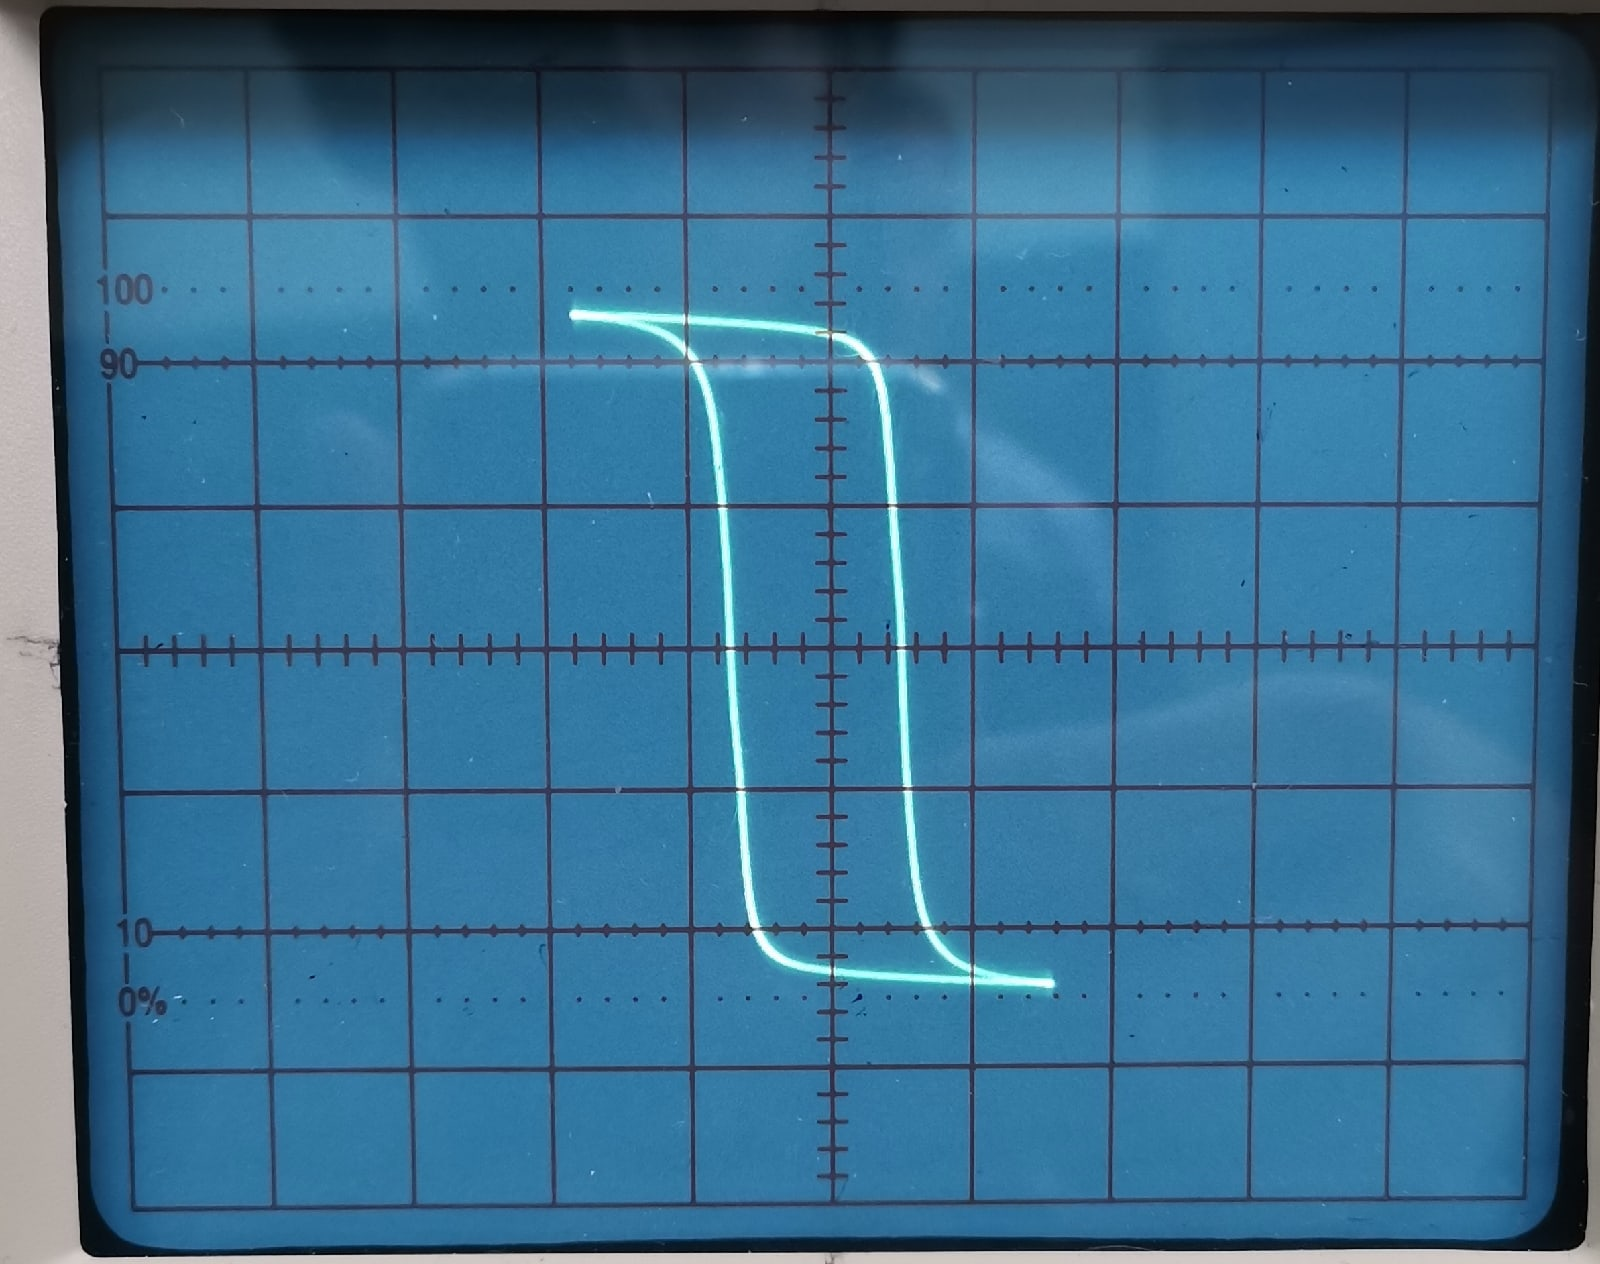
\includegraphics[width = 0.8\textwidth]{1.jpg}
\end{center}\
\textbf{Предельная кривая. Пермаллой}


\begin{center}
	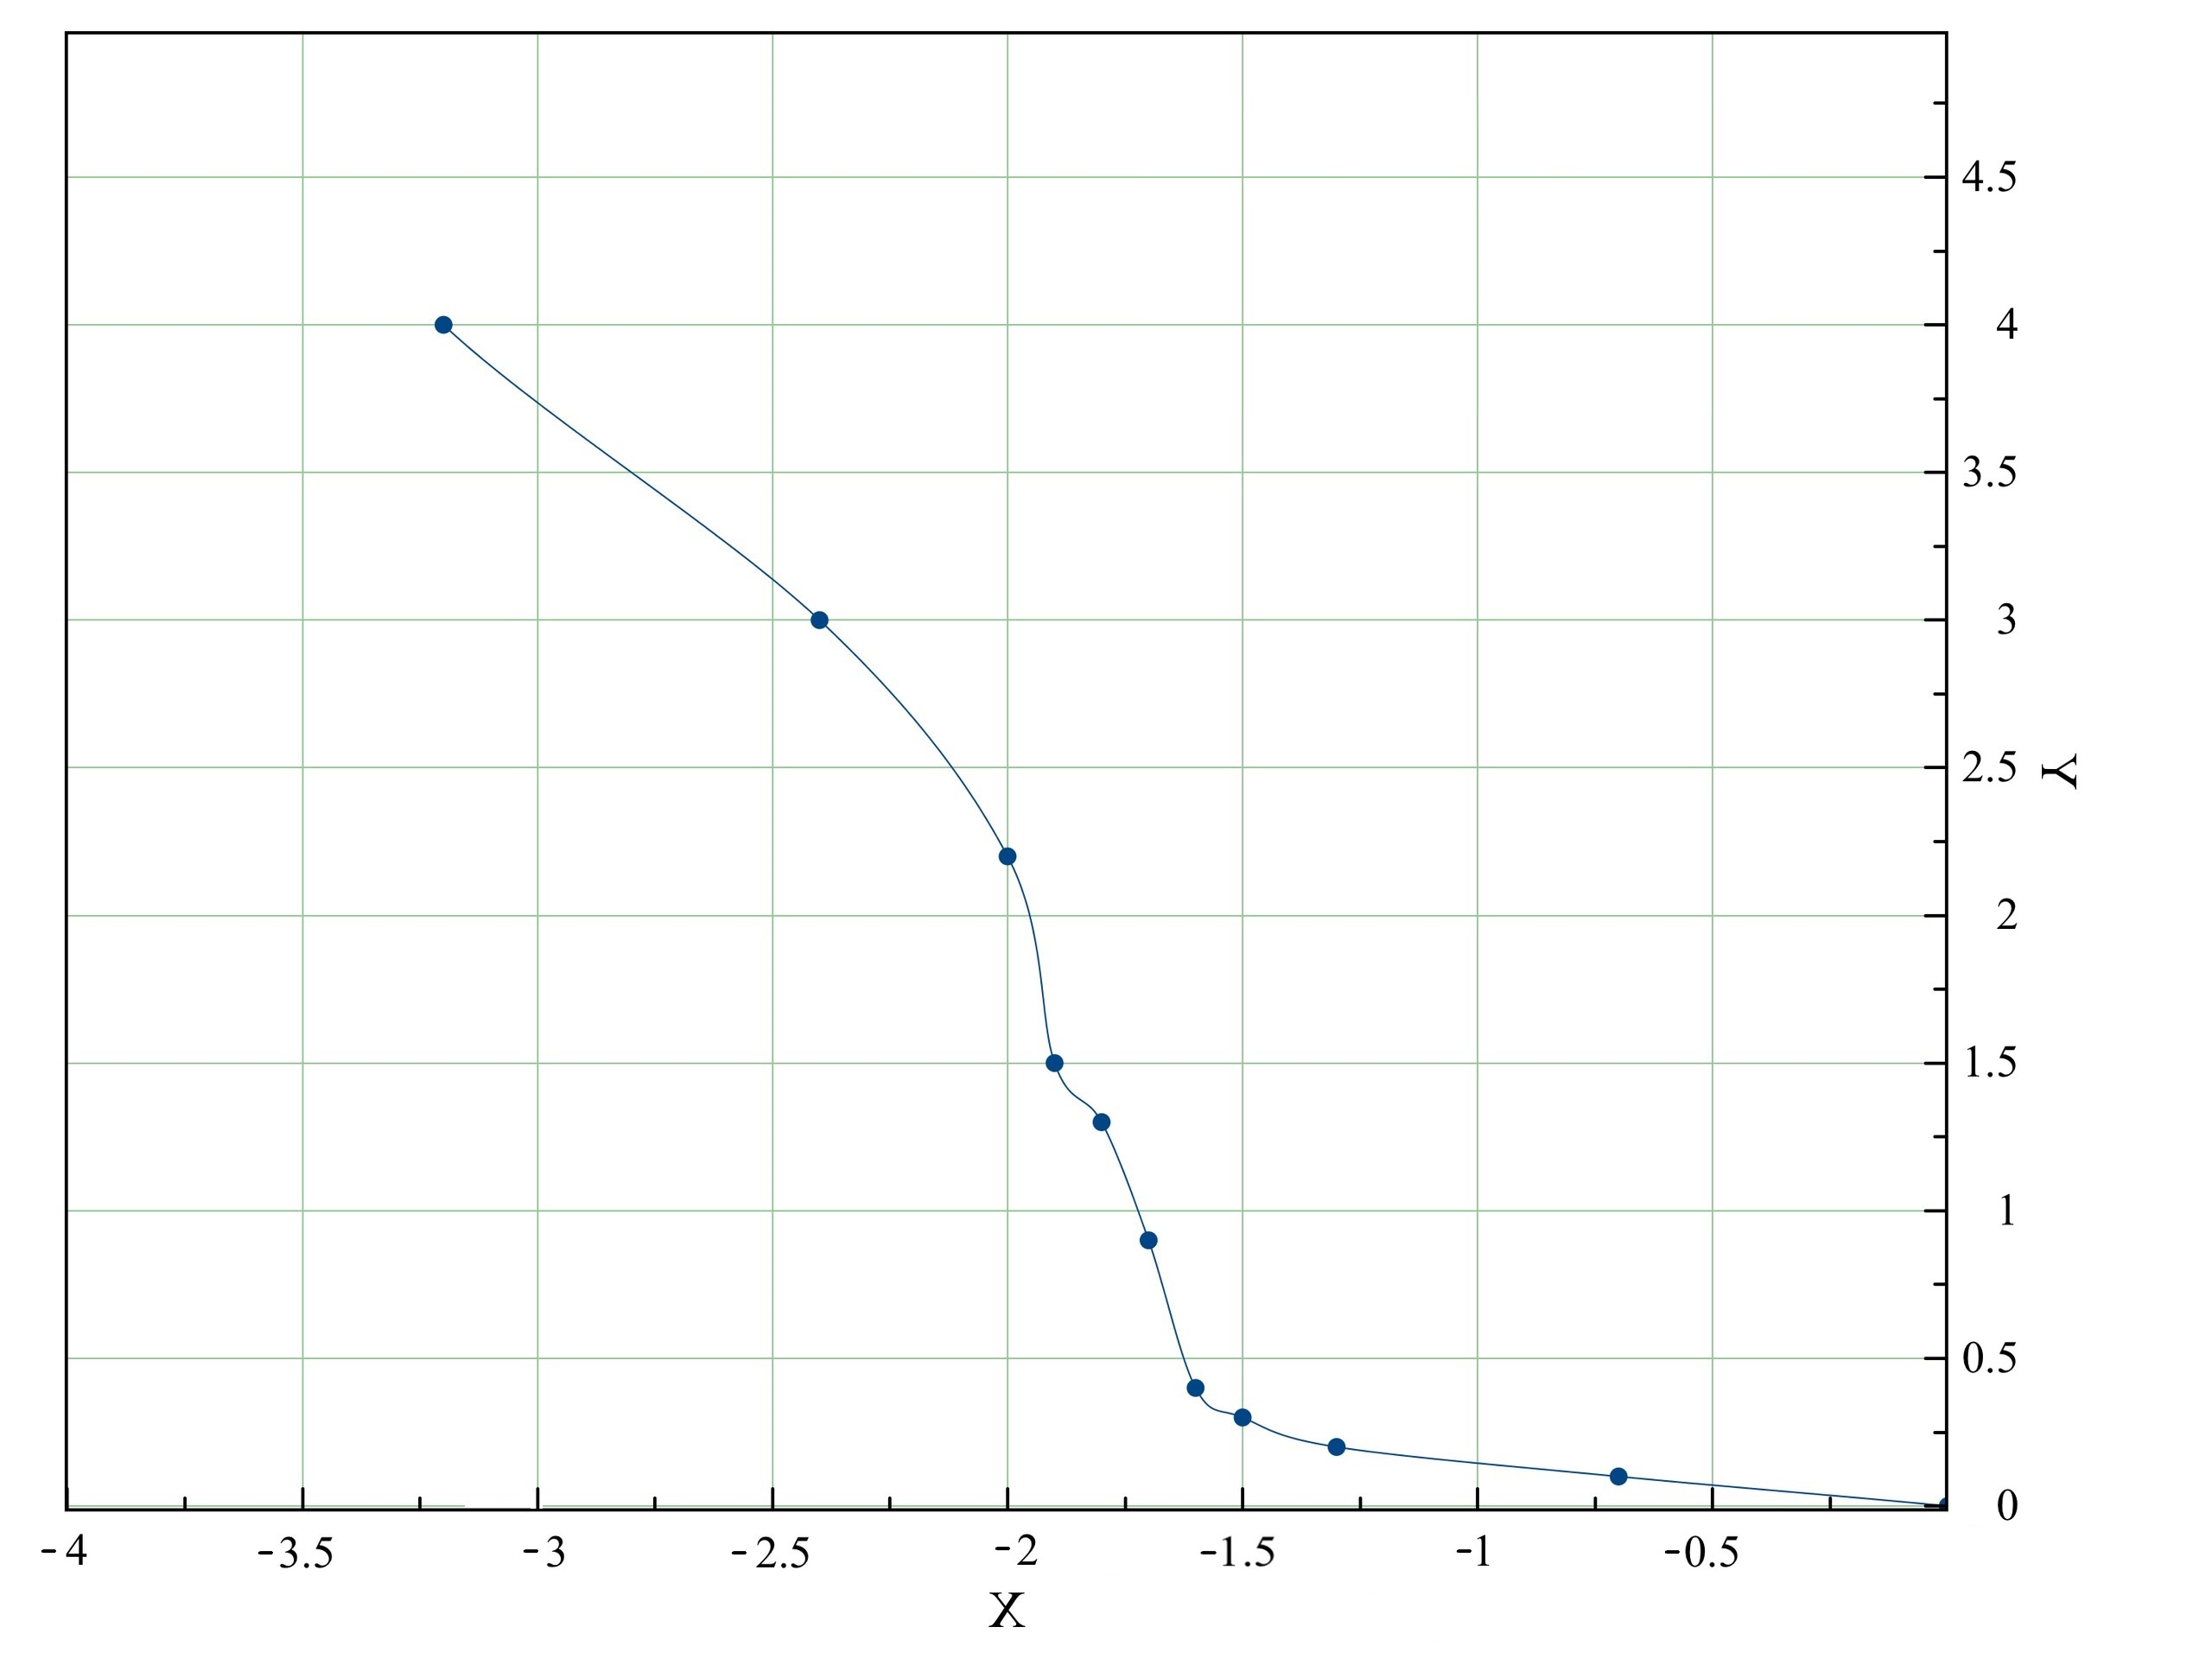
\includegraphics[width = 0.8\textwidth]{1_rev.jpg}
\end{center}\
\textbf{Начальная кривая. Пермаллой}

\newpage

\begin{center}
	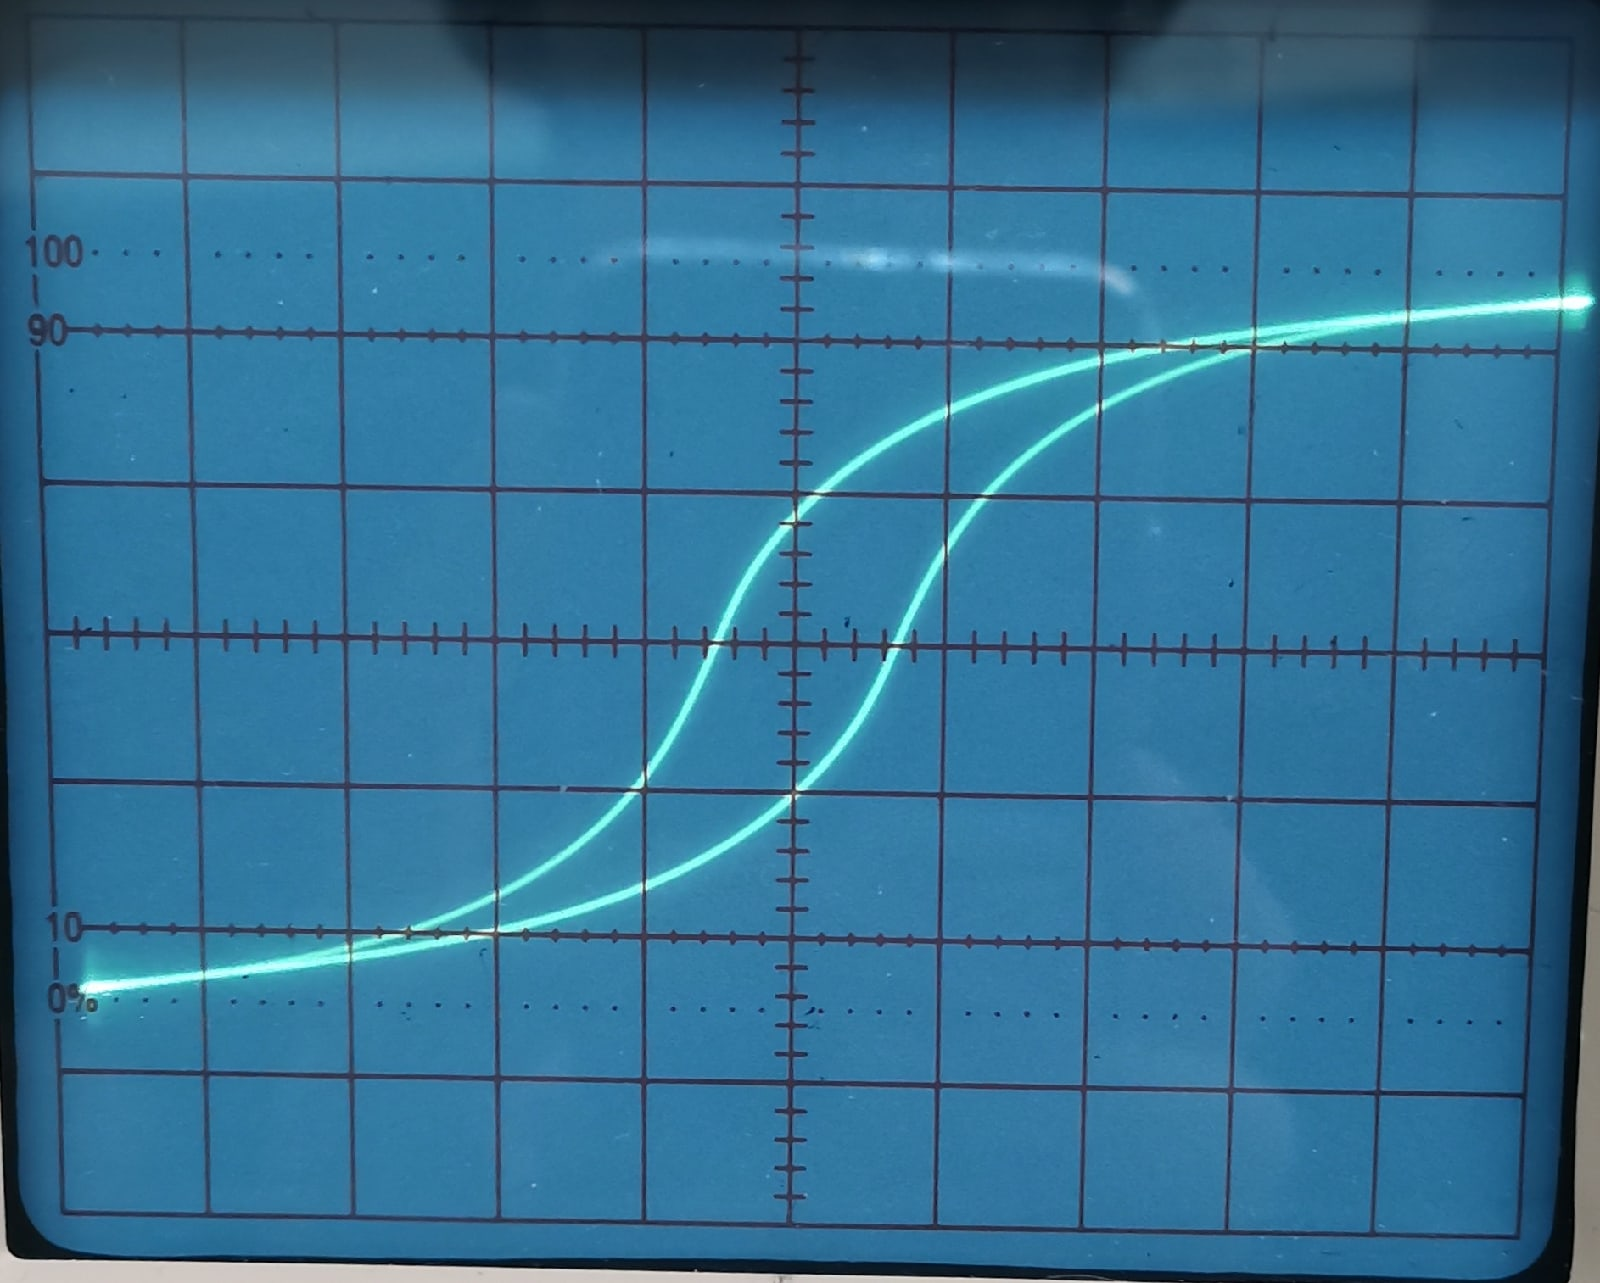
\includegraphics[width = 0.8\textwidth]{2.jpg}
\end{center}\
\textbf{Предельная кривая. Феррит}

\begin{center}
	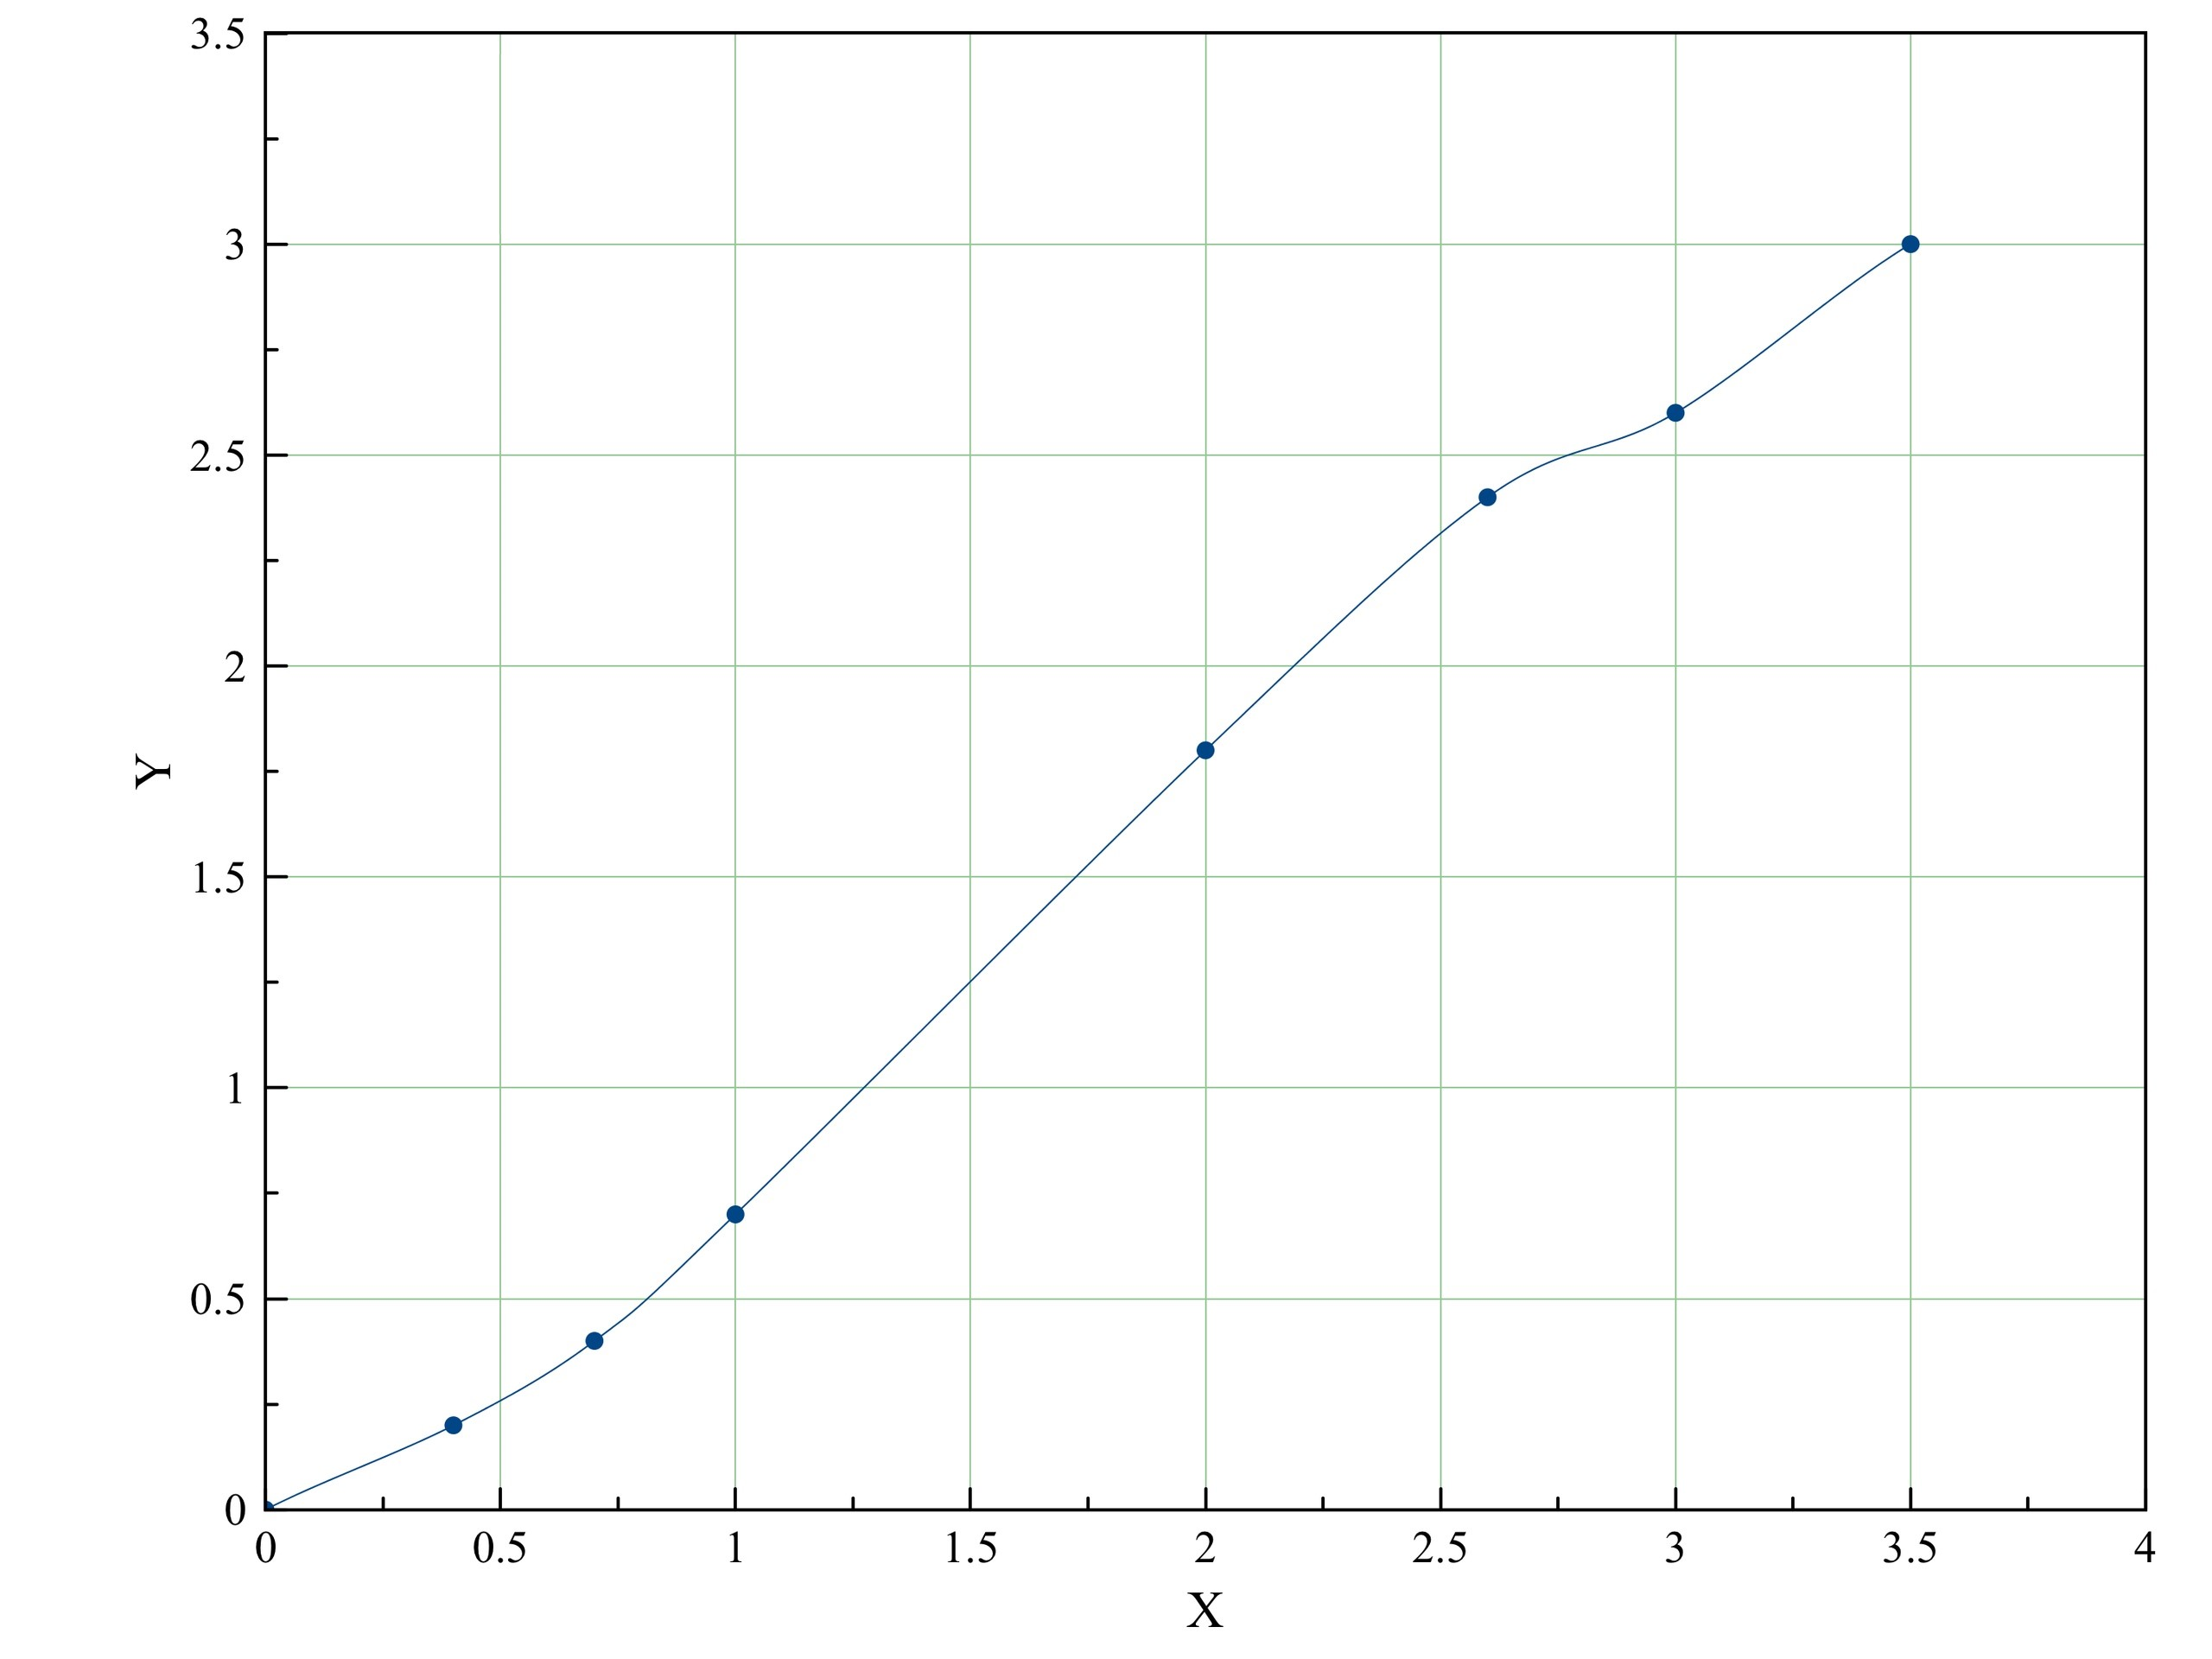
\includegraphics[width = 0.8\textwidth]{3_rev.jpg}
\end{center}\
\textbf{Начальная кривая. Феррит}

\newpage

\begin{center}
	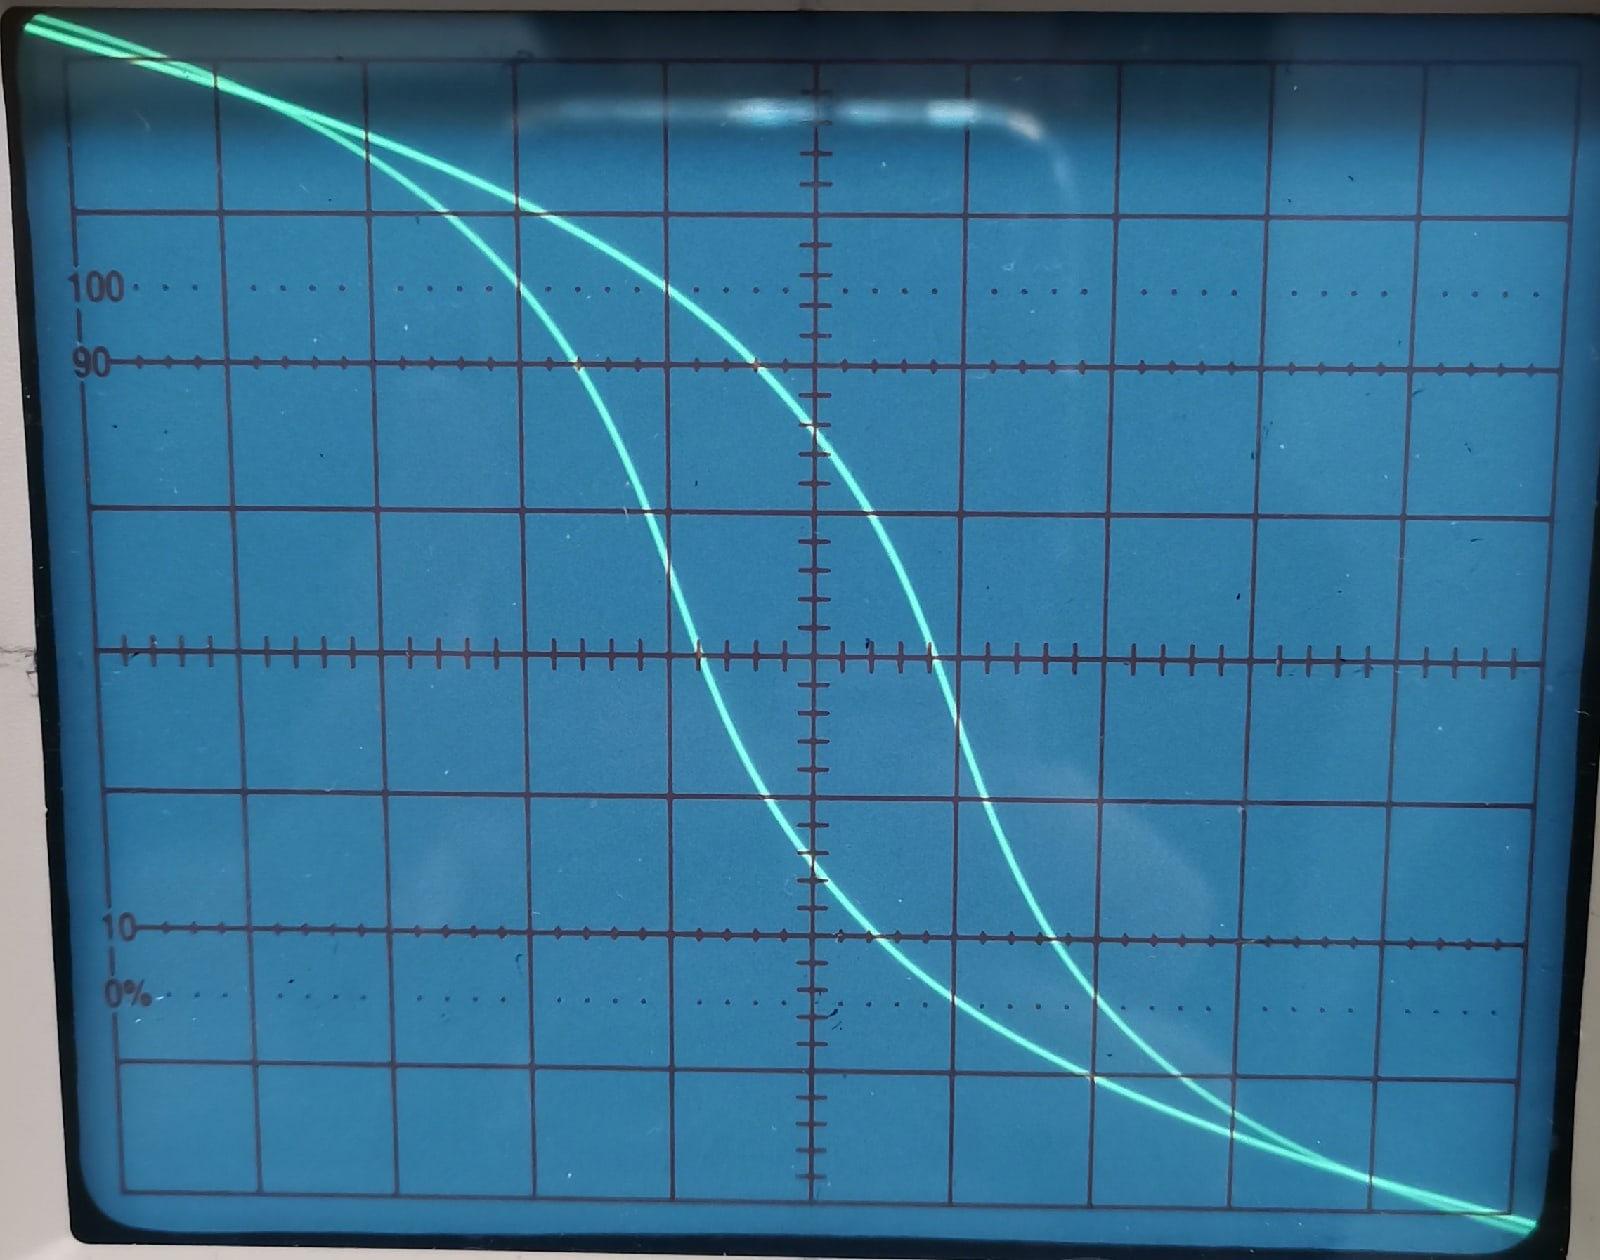
\includegraphics[width = 0.8\textwidth]{3.jpg}
\end{center}\
\textbf{Предельная кривая. Кремнистое железо}

\begin{center}
	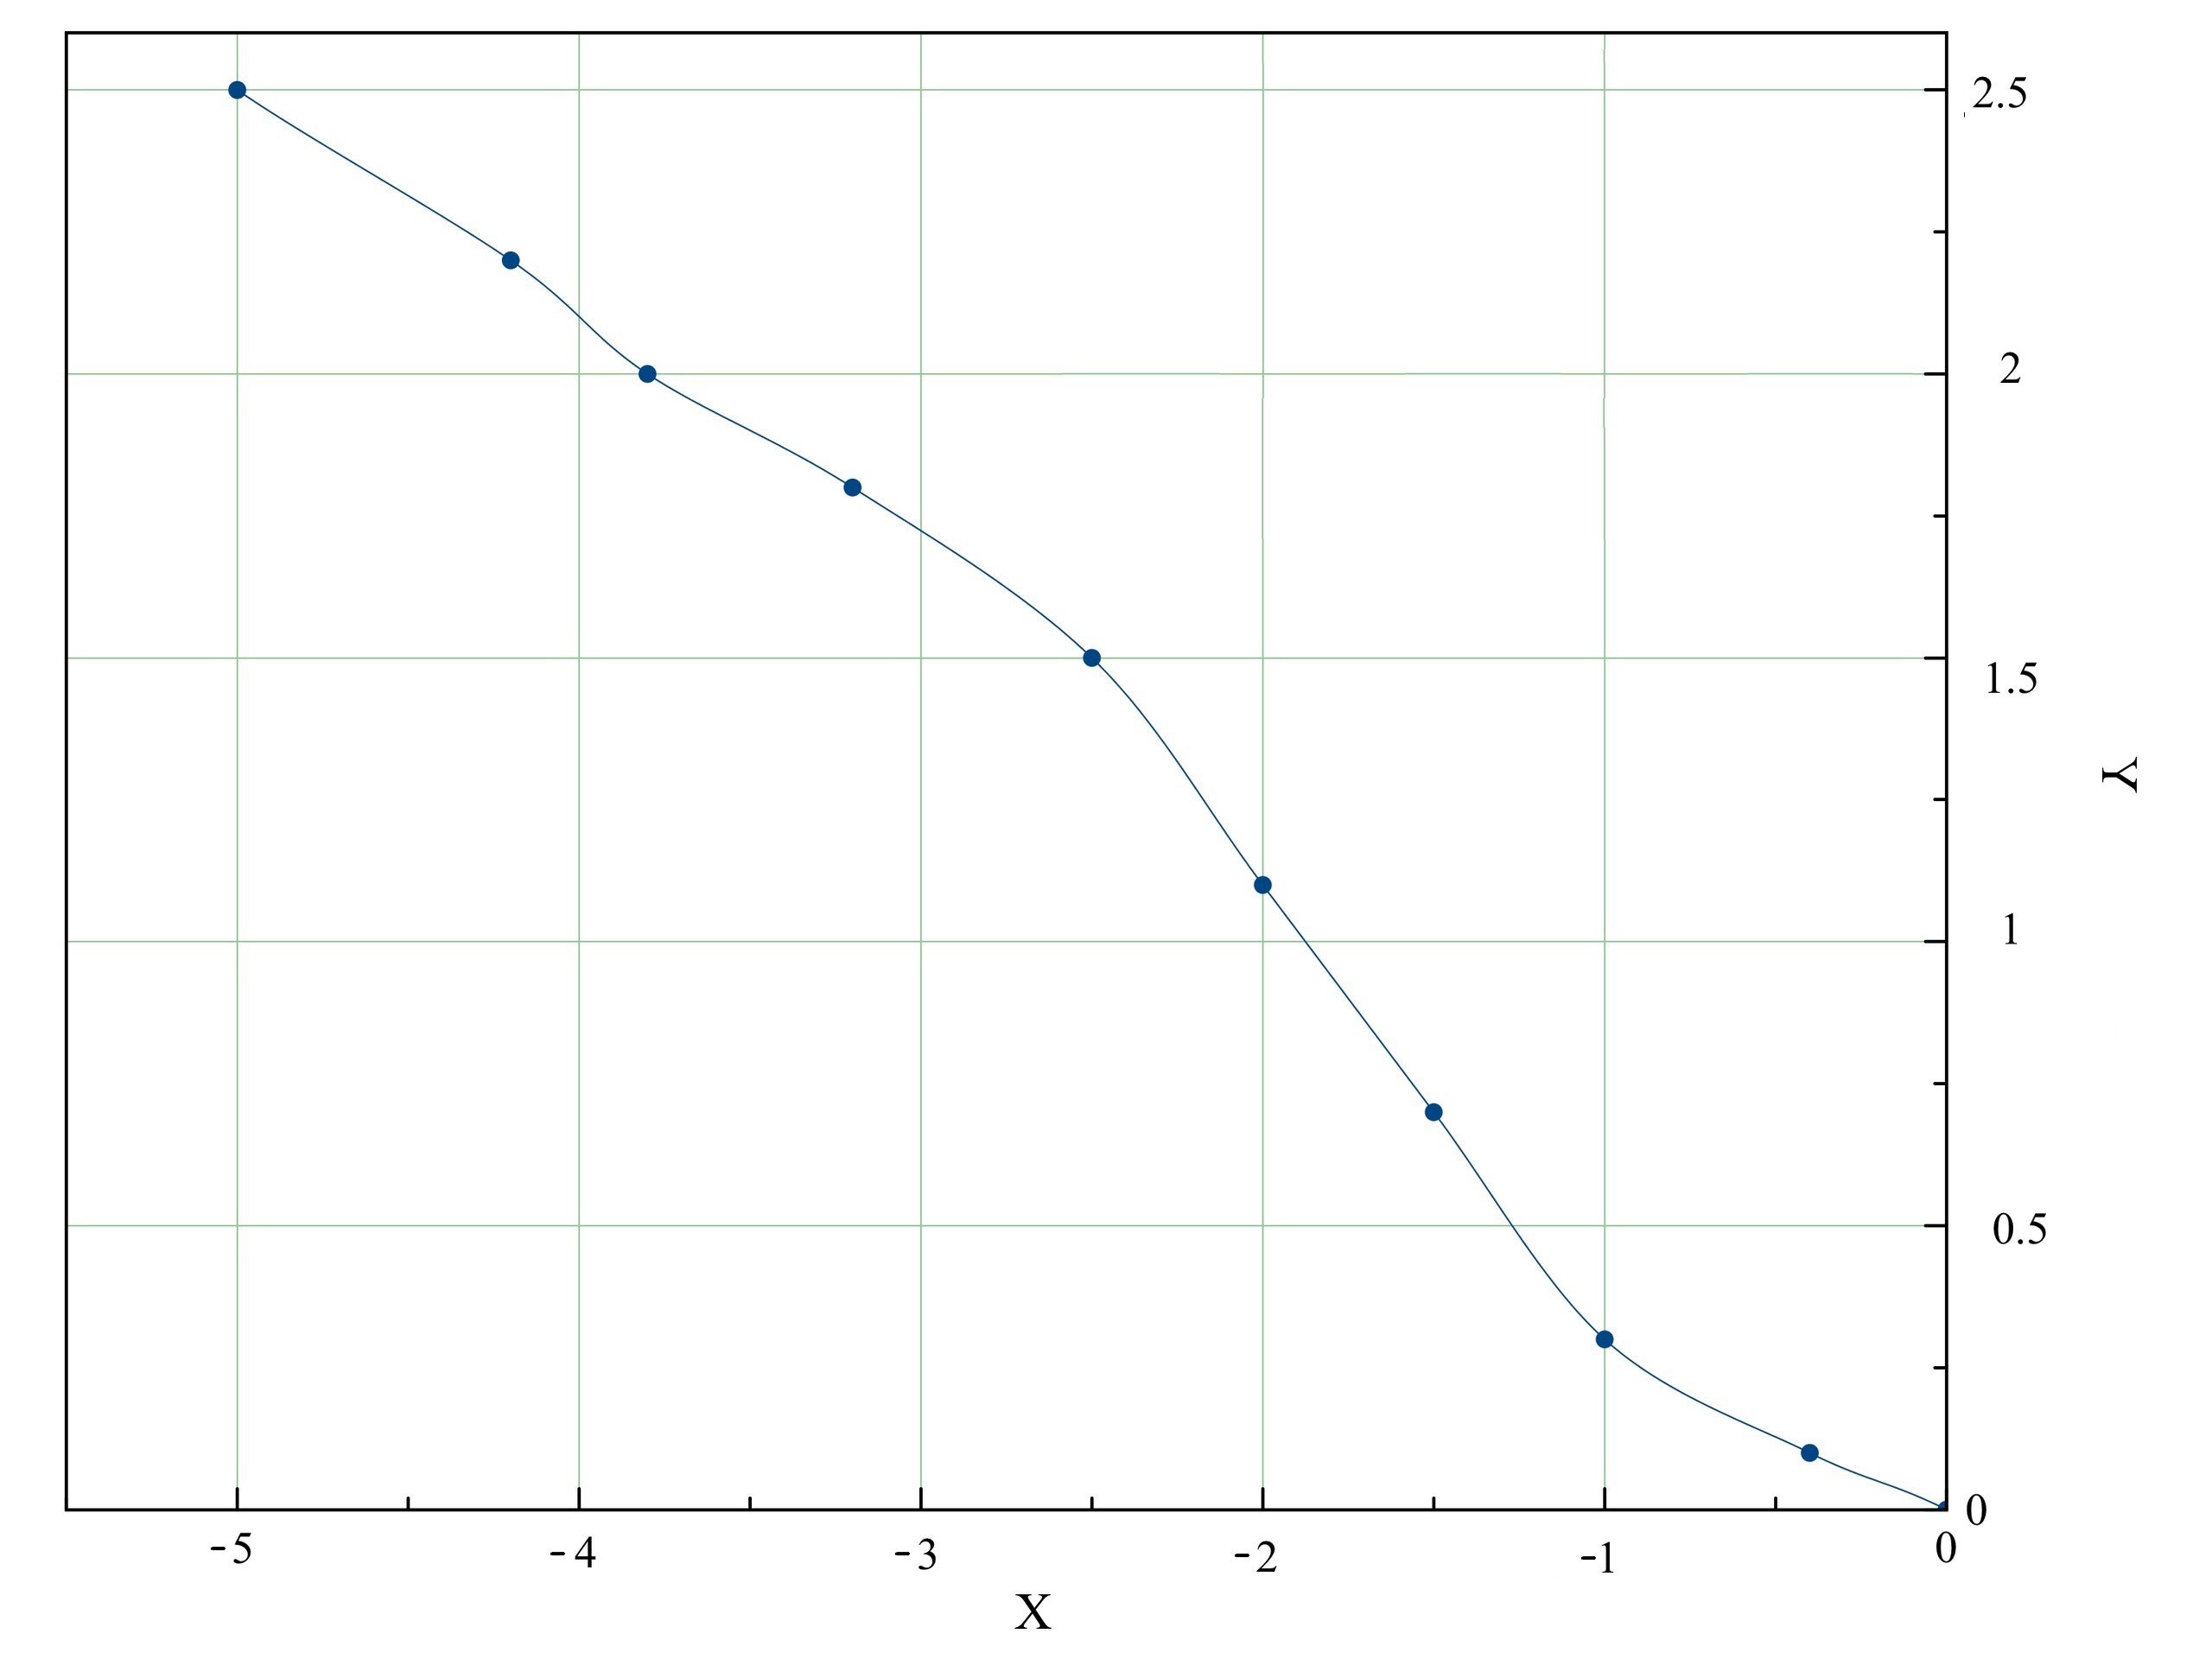
\includegraphics[width = 0.8\textwidth]{2_rev.jpg}
\end{center}\
\textbf{Предельная кривая. Кремнистое железо}

\subsection {Проверка калибровки оси X ЭО с помощью амперметра}


Отключим намагничивающую обмотку $N_0$ от цепи,  подберем такой ток через $R_0$ с помощью автотрансформатора, при котором горизонтальная прямая занимает большую часть экрана. Рассчитаем чувствительность канала $m_X$ по формуле и сравним с выбранным $K_X$.
\newline
Данные, полученные при измерении: $2x=7.0 $ , $I_{ef} = 155$ mA, $R_0 = 0.3$ Om, $K_x = 20 $ мВ.
\newline
Расчет:


$$m_x=\frac{2R_0\sqrt{2}I_{ef}}{(2x)}$$
$$m_x=\frac{2\cdot 0.3 \sqrt{2}\cdot 155}{7.5} \approx 19,4$$ 

\newline

Каллибровка проведена успешно.


\subsection {Проверка калибровки оси Y ЭО с помощью вольтметра}

Разберем цепь тороида; подберем c помощью автотрансформатора напряжение, при котором вертикальная прямая занимает большую часть экрана. Измерим двойную амплитуду сигнала. Определим эффективное значение напряжения. 
\newline
Данные, полученные при каллибровке:
$2y = 8$ делений, $U_{ef} = 0.13$ В, $K_y = 50$ мВ.
\newline

Рассчеты:

$$m_y=\frac{2\sqrt{2}U_{ef}}{(2y)}$$

$$m_y=\frac{2\sqrt{2} \cdot 130}{8} \approx 46$$

Каллибровка проведена успешно.

\subsection {Определение $\tau$ - постоянной времени $RC$-цепочки}


Определим напряжения на входе и выходе интегрирующей ячейки: подключим $Y$-вход и отключим $X$-вход; установим чувствительность $K_Y \approx n$ В/дел. подберем такой ток (с помощью реостата), при котором горизонтальная прямая занимает большую часть экрана. Определим входное напряжение на RC-цепочке. Переключим $Y$-вход ЭО к интегрирующей емкости и определим $U_{ex}$. Рассчитаем постоянную времени $\tau$.
\newline
Напряжение на входе ячейки $U_{in} = 2$ В, напряжение на выходе ячейки $U_{out} = 12$ mВ, $\Omega=50$ Гц.

С одной стороны:

$$\tau=R_uC_u=400 \: msec
$$

\newline

C другой стороны:


$$\tau=RC=\frac{U_{in}}{\Omega U_{ex}}=333 \: msec $$ .

Таким образом, проверили справедливость формул () и (), т.е. выполнение $\tau=RC \approx \frac{U_{in}}{\Omega U_{ex}}$$




\subsection{Дифференциальная магнитная проницаемость}



Вычислим максимальные значения дифференциальной магнитной проницаемости  для каждого из трех образцов по формуле:

\begin{equation}\label{}
    \mu_{dif}=\frac{1}{\mu_0}\frac{dB}{dH}
\end{equation}


где $\mu_0$ - магнитная постоянная ($\mu_0\approx1,256~ H/A^2$), а значение $\frac{dB}{dH}$ определим по графикам (максимальный наклон касательных к петлям гистерезиса, который достигается в точках с $B=0$, т.к. эти точки находятся наиболее далеко от областей насыщения).
\newline
Также рассчитаем $H_c, B_s$ по формулам (2), (3), учтя, что полученнеы значения необходимо домножить на число снятых делений.
\newline
Пусть $[2x(c)] = l_c$, $[2y(s)] = l_s$.
\newline
Также пусть $\sigma_R = 0.0005$ м, $\sigma_{l_c} = \frac{l_c}{10}$, аналогично $\sigma_{l_s} = \frac{l_s}{10}$, $\sigma_S = 2\sigma_r = 0.001$.
\newline
Погрешности $\sigma_{H_c} и \sigma_{B_s}$ рассчитаем по формулам:

\begin{equation}\label{}
\sigma_{H_s} = H_s\cdot\sqrt{(\frac{\sigma_R}{R})^2 + (\frac{\sigma_{l_c}}{l_c})^2}
\end{equation}


\begin{equation}\label{}
\sigma_{B_s} = B_s\cdot \sqrt{(\frac{\sigma_S}{S})^2 + (\frac{\sigma_{l_s}}{l_s})^2}
\end{equation}



Результаты занесем в итоговую таблицу. 

\begin{table}[h!]
	\centering
	\caption{Итоговые результаты}
    \begin{tabular}{|c|c|c|c|}
	\hline 
		& Кремнистое железо & Пермаллой & Феррит \\
		\hline 
		$H_c$, А/м & 172.8$\pm$8.6 & 44.6$\pm$2.2 & 67.2 $\pm$3.4\\
		\hline
		$B_s$, Тл &  1.25$\pm$0.06 & 0.20$\pm$0.01 & 0.080$\pm$0.004\\
		\hline
		$\mu_{\text{дифф}}^{\max}, \cdot \frac{1}{1000}$ & 9.8 & 50 & 2.7\\
        \hline
	    \end{tabular}% 
	    
\label{resT}% 
\end{table}% 



\section{Вывод}
Провели исследование петель гистерезиса трех ферромагнитных материалов(кремнистое железо, пермаллой и феррит). Для них мы построили начальные кривые гистерезиса для каждой из петель, нашли коэрцитивную силу и индукцию насыщения для каждого образца, оценили максимальные значения дифференциальной магнитной проницаемости для каждого образца, а также произвели калибровку осей ЭО и нашли постоянную $RC$-цепочки. Все экспериментально полученные результаты совпали с табличными кроме $H_c$ и $\mu_{\text{дифф}}^{\max}$ для Пермаллоя -- магнитная проницаемость достаточно меньше  табличного значения, вследствие чего, скорее всего не совпало и значения для $H_c$. Такое отклонение можно связать стем, что образец может быть довольно старым и изношенным, из-за чего у него и поменялись стандартные магнитные свойства. Полученные характеристики для данных материалов представляют практический интерес, т.к. часто используются в трансформаторах, дросселях, машинах переменного тока и пр.
\end{document}